\documentclass[a4paper,10pt]{book}
\usepackage[english]{babel}     
\usepackage[utf8]{inputenc}     % accent symbols
\usepackage[T1]{fontenc}
\usepackage{lmodern}
\usepackage{microtype}
\usepackage{natbib}
\usepackage{tocbibind}          
\usepackage{amsmath}            % math symbols
\usepackage{amsthm}             % math symbols
\usepackage[colorlinks=true,linkcolor=red]{hyperref} % hyper link

% for code
\usepackage{listings}
\usepackage{color,xcolor}
\definecolor{mygreen}{rgb}{0,0.6,0}
\definecolor{mygray}{rgb}{0.9,0.9,0.9}
\definecolor{mymauve}{rgb}{0.58,0,0.82}
\lstset{
backgroundcolor=\color{mygray},
numbers=left,                    
columns=fullflexible,
breaklines=true,      
captionpos=b,         
tabsize=4,            
commentstyle=\color{mygreen}, 
escapeinside={\%*}{*)},       
keywordstyle=\color{blue},    
% stringstyle=\color{mymauve}\monaco,
frame=single,                        
rulesepcolor=\color{red!20!green!20!blue!20},
% identifierstyle=\color{red},
%% language=c++,
basicstyle=\tiny
}

\usepackage{indentfirst}
\setlength{\parindent}{2em}
\usepackage[onehalfspacing]{setspace}
% graph
\usepackage{pdfpages}
\usepackage{graphicx}
% box
\usepackage{booktabs}
\usepackage{tcolorbox}

%% user defined command
\newcommand{\keyword}[1]{\textbf{#1}}
\newcommand{\keywords}[1]{\textbf{#1}}
\newcommand{\lcmd}[1]{\texttt{#1}}
\newcommand{\head}[1]{\textnormal{\textbf{#1}}}
\newcommand{\itwords}[1]{\textit{#1}}

\usepackage{float}
% all symbols
\usepackage{tipa}
\usepackage{tipx}

\usepackage{datetime}
% \usepackage{movie15}


% variable
% TODO
\newcommand{\pdfauthor}{李明明}
\newcommand{\pdftitle}{工作}
\newcommand{\pdfsubject}{工作中的经验与教训}
\newcommand{\pdfkeywords}{工作经验与教训}
\newcommand{\bookname}{工作收获}
\newcommand{\bookoneword}{工作中吸取的经验和教训}
\newcommand{\timeandcompany}{2020年12月1日}

\usepackage{bm}
\usepackage{amsfonts}
\begin{document}


% Pages are numbered with lowercase Roman numbers.
% Chapters generate a table of contents entry but don't get a number.
\frontmatter{}
\newcommand{\mytitle}{Git}
\newcommand{\firstcreated}{Mar 16, 2023}

\begin{titlepage}

\newcommand{\HRule}{\rule{\linewidth}{0.5mm}} % Defines a new command for the horizontal lines, change thickness here

\center                         % Center everything on the page
 
%----------------------------------------------------------------------------------------
%	HEADING SECTIONS
%----------------------------------------------------------------------------------------


\includegraphics[width=0.5\textwidth]{logo}\\[1cm] % Include a department/university logo - this will require the graphicx package

%----------------------------------------------------------------------------------------
%	TITLE SECTION
%----------------------------------------------------------------------------------------

\HRule\\[0.4cm]
{ \huge \bfseries \mytitle}\\[0.4cm] % Title of your document
\HRule\\[1.5cm]
 
%----------------------------------------------------------------------------------------
%	AUTHOR SECTION
%----------------------------------------------------------------------------------------

\begin{minipage}{0.4\textwidth}
\begin{center} \large
Mingming \textsc{Li}\\ % Your name
\end{center}

\end{minipage}\\[2cm]


%----------------------------------------------------------------------------------------
%	DATE SECTION
% ----------------------------------------------------------------------------------------
\vfill
{\large First Created: \firstcreated}\\
{\large Last Modified: \today}\\[2cm] % Date, change the \today to a set date if you want to be precise



\end{titlepage}


%%% Local Variables:
%%% mode: latex
%%% Tex-master: "git"
%%% End:
\cleardoublepage{}
\phantomsection{}
\tableofcontents{}
\cleardoublepage{}
\phantomsection{}
\listoffigures{}
\cleardoublepage{}
\phantomsection{}
\listoftables{}


% Pages are numbered with Arabic numbers.
% Chapters are numbered and produce a table of contents entry.
\mainmatter{}

\part{Theory}
\label{part:theory}

\chapter{Math Formulas}
\label{cha:math-formulas}

\section{Math Mode}
\label{sec:math-mode}

Using math environments to enter math mode.

\subsection{Embedding Math Expressions Within Text}
\label{sec:embedd-math-expr}

LaTeX provides the math environment in-text formulas:
\begin{lstlisting}
\begin{math}
  expression
\end{math}
\end{lstlisting}


Since it's very laborious to write this environment for each small expression or symbol, LaTeX offers an alias that's doing the same:
\begin{lstlisting}
\(
expression
\)
% or
\(expression\)
\end{lstlisting}

A third way is by using a shortcut, coming from TeX:
\begin{lstlisting}
$expression$
\end{lstlisting}

\subsection{Displaying Formulas}
\label{sec:displaying-formulas}

For displayed formulas, which have to be centered, LaTeX offers the displaymath environment:
\begin{lstlisting}
\begin{displaymath}
  expression
\end{displaymath}
\end{lstlisting}

The effect of this environment is that the paragraph will be ended, some vertical space follows, then the centered formula plus the following vertical space.
As this math environment takes care of the spacing, don't leave empty lines before and after it!
This would cause additional vertical space because of the superfluous paragraph breaks.

A shortcut is:
\begin{lstlisting}
\[
expression
\]
\end{lstlisting}

\subsection{Numbering Equations}
\label{sec:numbering-equations}

Equations and formulas in general may be numbered.
However, this applies only to displayed formulas.
The equation environment is responsible for this:
\begin{lstlisting}
\begin{equation}
  \label{key}
  expression
\end{equation}
\end{lstlisting}

\section{Common Formulas}
\label{sec:common}

\begin{table}[H]
  \centering
  \begin{tabular}{ll}
    \toprule
    \head{Source code} & \head{Output}\\
    \midrule
    \lstinline|x^2| & $x^{2}$ \\
    \lstinline|x_2| & $x_{2}$ \\
    \lstinline|\sqrt[3]{x}| & $\sqrt[3]{x}$\\
    \lstinline|\frac{x}{y}| & $\frac{x}{y}$\\
    \bottomrule
  \end{tabular}
  \caption{Common}
  \label{tab:common}
\end{table}


\section{Dots}
\label{sec:dots}

\begin{table}[H]
  \centering
  \begin{tabular}{>{\textbackslash\ttfamily}ll}
    \toprule
    \normal{\head{Source code}} & \head{Output}\\
    \midrule
    ddots & $\ddots$\\
    cdot & $\cdot$\\
    ldots & $\ldots$\\
    vdots & $\vdots$\\
    dot\{\} & $\dot{}$\\
    cdots & $\cdots$\\
    \bottomrule
  \end{tabular}
  \caption{Dots}
  \label{tab:dots}
\end{table}


\section{Greek Letters}
\label{sec:greek-letters}

To get a lowercase Greek letter, just write the name with a backslash for the command.

\begin{table}[H]
  \centering
  \begin{tabular}{>{\textbackslash\ttfamily}ll>{\textbackslash\ttfamily}ll}
    \toprule
    \normal{\head{Source code}} & \head{Output} & \normal{\head{Source code}} & \head{Output}\\
    \midrule
    alpha & $\alpha$ & beta & $\beta$\\
    gamma & $\gamma$ &  delta & $\delta$\\
    epsilon & $\epsilon$ & zeta & $\zeta$\\
    eta & $\eta$ & theta & $\theta$\\
    iota & $\iota$ & kappa & $\kappa$\\
    lambda & $\lambda$ & mu & $\mu$\\
    nu & $\nu$ & xi & $\xi$\\
    \normal{o} & o & pi & $\pi$\\
    rho & $\rho$ & sigma & $\sigma$\\
    tau & $\tau$ & upsilon & $\upsilon$\\
    phi & $\phi$ & chi & $\chi$\\
    psi & $\psi$ & omega & $\omega$\\
    \midrule
    varepsilon & $\varepsilon$ & vartheta & $\vartheta$\\
    varpi & $\varpi$ & varrho & $\varrho$\\
    varsigma & $\varsigma$ & varphi & $\varphi$\\
    \midrule
    Gamma & $\Gamma$ & Delta & $\Delta$\\
    Theta & $\Theta$ & Lambda & $\Lambda$\\
    Xi & $\Xi$ & Pi & $\Pi$\\
    Sigma & $\Sigma$ & Upsilon & $\Upsilon$\\
    Phi & $\Phi$ & Psi & $\Psi$\\
    Omega & $\Omega$\\
    \bottomrule
  \end{tabular}
  \caption{Greek Letters}
  \label{tab:greek-letters}
\end{table}




\section{Fonts}
\label{sec:fonts}

\begin{table}[H]
  \centering
  \begin{tabular}{>{\textbackslash{}\ttfamily{}}l<{\{...\}}ll}
    \toprule
    \normal{\head{Source code}} & \head{Package} & \head{Output}\\
    \midrule
    mathrm &  & $\mathrm{abc\ 123}$\\
    mathit & & $\mathit{abc\ 123}$\\
    mathsf & & $\mathsf{abc\ 123}$\\
    mathbb & amsfonts & $\mathbb{ABC}$\\
    mathbbm & bbm & $\mathbbm{ABC}$\\
    mathds & dsfont & $\mathds{ABC}$\\
    mathfrak & eufrak & $\mathfrak{ABC\ 123}$\\
    mathnormal & & $\mathnormal{ABC\ 123}$\\
    \bottomrule
  \end{tabular}
  \caption{Fonts}
  \label{tab:fonts}
\end{table}

\section{Multi-line Formulas}
\label{sec:multi-line-formulas}

\begin{lstlisting}
% package amsmath needed
\begin{multline}
\sum = a + b + c + d + e \\
           + f + g + h + i + j \\
           + k + l + m + n 
\end{multline}


\begin{gather}
x + y + z = 0 \\ 
y-z= 1
\end{gather}


\begin{align}
  x + y + z &= 0 \\
  y - z &= 1
\end{align}
\end{lstlisting}


\begin{multline}
\sum = a + b + c + d + e \\
           + f + g + h + i + j \\
           + k + l + m + n 
\end{multline}


\begin{gather}
x + y + z = 0 \\ 
y-z= 1
\end{gather}


\begin{align}
  x + y + z &= 0 \\
  y - z &= 1
\end{align}

\section{Operators}
\label{sec:operators}

Trigonometric functions, logarithm functions, and other analytic and algebraic functions are commonly written with upright Roman letters.
Simply typing log would otherwise look like a product of the three variables, namely, l, o, and g.
To ease the input, there are commands for many common functions or so called \keyword{operators}.
Here's an alphabetical list of the predefined ones:
\begin{lstlisting}
\arccos, \arcsin, \arctan, \arg, \cos, \cosh, \cot, \coth, \scs, \deg, \det, \dim, \exp, \gcd, \hom, \inf, \ker, \lg, \lim, \liminf, \limsup, \ln, \log, \max, \min, \Pr, \sec, \sin, \sinh, \sup, \tan, \tanh
\end{lstlisting}

\newpage{}
\section{Standard LaTeX Symbols}
\begin{table}[H]
  \centering
  \begin{tabular}{>{\textbackslash\ttfamily}ll>{\textbackslash{}\ttfamily{}}ll}
    \toprule
    \normal{\head{Source code}} & \head{Output} & \normal{\head{Source code}} & \head{Output}\\
    \midrule
    circ & $\circ$ & bigcirc & $\bigcirc$\\
    star & $\star$ & ast & $\ast$\\
    cup & $\cup$ & cap & $\cap$\\
    ominus & $\ominus$ & oplus & $\oplus$\\
    oslash & $\oslash$ & otimes & $\otimes$\\
    times & $\times$ & div & $\div$\\
    pm & $\pm$ & mp & $\mp$\\
    odot & $\odot$ & bullet & $\bullet$\\
    \midrule
    approx & $\approx$ & equiv & $\equiv$\\
    propto & $\propto$ & sim & $\sim$\\
    simeq & $\simeq$\\
    parallel & $\parallel$ & perp & $\perp$\\
    subset & $\subset$ & supset & $\supset$\\
    subseteq & $\subseteq$ & supseteq & $\supseteq$\\
    \midrule
    geq & $\geq$ & gg & $\gg$\\
    leq & $\leq$ & ll & $\ll$\\
    neq & $\neq$\\
    \midrule
    prod & $\prod$ & sum & $\sum$ \\
    coprod & $\coprod$ & int & $\int$\\
    oint & $\oint$\\
    \midrule
    rightarrow & $\rightarrow$ & Rightarrow & $\Rightarrow$\\
    longrightarrow & $\longrightarrow$ & Longrightarrow & $\Longrightarrow$\\
    hookleftarrow & $\hookleftarrow$ & hookrightarrow & $\hookrightarrow$\\
    leftrightarrow & $\leftrightarrow$ & Leftrightarrow $\Longleftrightarrow$\\
    \midrule
    bot & $\bot$ & forall & $\forall$\\
    ni & $\ni$ & top & $\top$\\
    hbar & $\hbar$ & in & $\in$\\
    exists & $\exists$ \\
    \midrule
    langle & $\langle$ & lceil & $\lceil$\\
    lfloor & $\lfloor$ & | & $\|$\\
    \midrule
    sharp & $\sharp$ & nabla & $\nabla$\\
    emptyset & $\emptyset$ & angle & $\angle$\\
    flat & $\flat$ & neg & $\neg$\\
    surd & $\surd$ & infty & $\infty$\\
    prime & $\prime$ & triangle & $\triangle$\\
    \bottomrule
  \end{tabular}
  \caption{Standard latex sysmbols}
  \label{tab:standard-latex-symbols}
\end{table}

\section{Math Structures}
\label{sec:math-structures}

\begin{lstlisting}
\[
\binom{n}{k} = \frac{n!}{k!(n-k)!}
\]
\end{lstlisting}

\[
\binom{n}{k} = \frac{n!}{k!(n-k)!}
\]


\begin{lstlisting}
\[
A = 
\begin{pmatrix}
  a_{11} & a_{12} \\
  a_{21} & a_{22}
\end{pmatrix}
\]
\end{lstlisting}

\[
A =
\begin{pmatrix}
  a_{11} & a_{12} \\
  a_{21} & a_{22}
\end{pmatrix}
\]

These are amsmath's matrix environments:

\begin{table}[H]
  \centering
  \begin{tabular}{>{\ttfamily}ll}
    \toprule
    \normal{\head{Name}} & \head{Delimiters of the matrix}\\
    \midrule
    matrix & no delimiters\\
    pmatrix & parentheses()\\
    bmatrix & square brackets[]\\
    Bmatrix & braces\{\}\\
    vamtrix & $|$\\
    Vmatrix & $\|$$\|$\\
    smallmatrix & without delimiters, add them if needed, more compact\\
    \bottomrule
  \end{tabular}
  \caption{Matrix}
  \label{tab:matrix}
\end{table}

\section{Stakcing Expressions}
\label{sec:stakcing-expressions}

\subsection{Underlining and Overlining}
\label{sec:underl-overl}

\begin{lstlisting}
\[s = \overline{AB}\]
\[s = \underline{AB}\]
\[N = \underbrace{1 + 1 + \cdots + 1}_n\]
\[N = \overbrace{1 + 1 + \cdots + 1}_n\]
\end{lstlisting}
\[s = \overline{AB}\]
\[s = \underline{AB}\]
\[N = \underbrace{1 + 1 + \cdots + 1}_n\]
\[N = \overbrace{1 + 1 + \cdots + 1}_n\]

\subsection{Setting Accents}
\label{sec:setting-accents}

\begin{table}[H]
  \centering
  \begin{tabular}{>{\textbackslash\ttfamily}l<{\{a\}}l>{\textbackslash{}\ttfamily{}}l<{\{a\}}l}
    \toprule
    \normal{\head{Source code}} & \head{Output} & \normal{\head{Source code}} & \head{Output}\\
    \midrule
    bar & $\bar{a}$ & acute & $\acute{a}$\\
    check & $\check{a}$ & grave & $\grave{a}$\\
    tilde & $\tilde{a}$ & ddot & $\ddot{a}$\\
    hat & $\hat{a}$ & vec & $\vec{a}$\\
    breve & $\breve{a}$ & dot & $\dot{a}$\\
    mathring & $\mathring{a}$\\
    widehat & $\widehat{abc}$ & widetilde & $\widetilde{a}$\\
    \bottomrule
  \end{tabular}
  \caption{Accents}
  \label{tab:accents}
\end{table}


\subsection{Puting a Symbol Above Another}
\label{sec:puting-symbol-above}

\begin{lstlisting}
% package amsmath

\[\underset{A}{\equiv}\]
\[\overset{\equiv}{A}\]
\end{lstlisting}

\[\underset{A}{\equiv}\]
\[\overset{\equiv}{A}\]

%%% Local Variables:
%%% mode: latex
%%% TeX-master: "latex"
%%% End:


\chapter{Learning}
\label{cha:learning}

A machine learning algorithm is an algorithm that is able to learn from data.
But what do we mean by learning?
Mitchell provides a succinct definition:
``A computer program is said to learn from experience $E$ with respect to some class of tasks $T$ and performance measure $P$, if its performance at tasks in $T$, as measured by $P$, improves with experience $E$''


Now, how does the learn happen?
The model or algorithm learns by adjusting the parameters contained in it.

How to adjust the parameters?
Refer to Chapter \ref{cha:training}.


%%% Local Variables:
%%% mode: latex
%%% TeX-master: "machine-learning"
%%% End:


\chapter{Model}
\label{cha:model}

What is a model?

You can think a model as a function in math.
For example,
\begin{equation*}
  ax + by = c
\end{equation*}
In this function, \(a, b\) and \(d\) are the parameters, \(x\) and \(y\) are input from data.
Through adjusting the parameters \(a, b\) and \(d\), we can implement the learning process.
This is also called training in machine learning.

\section{Capacity}
\label{sec:capacity}

The capacity is the function space.
It defines the limitation that can learn from data.

For example,
\begin{equation*}
  ax + by = c  
\end{equation*}
This function can only learn linear function from data.
\begin{equation*}
  ax_{1}^{2} + bx_{2} = c
\end{equation*}
This function can learn curve function from data.


\subsection{The no free lunch theorem}


For any algorithms (functions) \(a_{1}\) and \(a_{2}\), at iteration step \(m\)
\begin{equation}
  \label{eq:1}
  \sum P(d_{m}^{y}|f,m,a_{1}) = \sum P(d_{m}^{y}|f,m,a_{2})
\end{equation}
where \(d_{m}^{y}\) denotes the ordered set of size \(m\) of the cost values \(y\) associated to input values \(x \in X\), \(f:X\longrightarrow Y\) is the function being optimized and \(P(d_{m}^{y}|f,m,a)\) is the conditional probability of obtaining a given sequence of cost values from algorithm \(a\) run \(m\) times on function \(f\).

The no free lunch theorem implies that we must design our machine learning algorithms to perform well on a specific task but not a universal task.

\subsection{Universal approximation theorem}
\label{sec:univ-appr-theor}

A feed-forward network with a single hidden layer containing a finite number of neurons can
approximate continuous functions on compact subsets of $R^n$ , under mild assumptions on the activation function. 

Let $\varphi$ : R $\rightarrow$ R be a nonconstant, bounded, and continous functions.
Let $I_m$ denote the m-dimensional unit hypercube $[0,1]^m$ .
The space of real-value continous function on $I_m$ is denoted by $C(I_m)$ .
Then, given any $\varepsilon > 0$ and function $f \in C(I_m)$ ,
there exist an integer N, real constants $\upsilon_i, b_i \in R$ and real vectors $\omega_i \in R^m$ for $i = 1, \cdots, N$ , such that we may define:
\begin{equation}
F(x) = \sum_{i=1}^{N}\upsilon_i\varphi(\omega_i^Tx+b_i)
\end{equation}
as an approximate realization of the function f; that is
\begin{equation}
|F(x) - f(x)| < \varepsilon
\end{equation}
for all $x \in I_m$ .
In other words, functions of the form $F(x)$ are dense in $C(I_m)$ .

This still holds when replacing $I_m$ with any compact subset of $R^m$ .



Kurt Hornik showed in 1991 that it is not the specific choice of the activation function, but rather the multilayer feedforward architecture itself which gives neural networks the potential of being universal approximators. The output units are always assumed to be linear. For notational convenience, only the single output case will be shown. The general case can easily be deduced from the single output case.

In 2017 Lu et al. proved universal approximation theorem for width-bounded deep neural networks.

This is the base of deep learning.

\section{Overfitting and underfitting}


We train model on training data but use test data (not used to train the model) to test out model.
The ability to perform on test data is called \keyword{generalization}.
We can use model on test data because we assume that the train data and the test has the same probability distribution (i.e. they have relationship).

The error on training data is called \keyword{training error}.
The error on test data is called \keyword{test error}.
Underfitting occurs when the model is not able to obtain a sufficient low error value on the training set.
Overfitting occurs when the gap between the training error and test error is too large.


We can control whether a model is more likely to overfit or underfit by altering its \keyword{capacity}.
The overfitting and underfitting happen because of the mismatch of capacity and the data.


%%% Local Variables:
%%% mode: latex
%%% TeX-master: "machine-learning"
%%% End:


\chapter{Training (optimization)}
\label{cha:training}

Training is the process of learning.
By inputting the data, we adjust the parameters in the model to achieve better performance.
In machine learning this is also called the optimization.


\section{SGD}
\label{sec:sgd}
Stochastic gradient descent (SGD) is a very basic and important algorithm.

The cost function used by a machining learning algorithm often decomposes as a sum over training examples of some per-example loss function.

\begin{equation}
  J(\bm{\theta}) = \mathbb{E}_{\mathrm{x},y \sim \hat{p}_{data}} L(\bm{x},y,\bm{\theta}) = \frac{1}{m}\sum_{i=1}^m L(\bm{x}^{(i)},y^{(i)},\bm{\theta}),
\end{equation}

Where \(L\) is the loss function, \(x\) and \(y\) are the input data and labels, \(\theta\) is the parameters in the model, \(m\) is the number of samples.


The gradient is
\begin{equation}
  \nabla_{\bm{\theta}} J(\bm{\theta}) = \frac{1}{m}\sum_{i=1}^m L(\bm{x}^{(i)},y^{(i)},\bm{\theta}).
\end{equation}

The computational cost of this operation is $O(m)$.
As the training set size grows to billions of examples, the time to take a single gradient step becomes prohibitively long.

The insight of SGD is that the gradient is an expectation.
The expectation may be approximately estimated using a small set of samples.
Specifically, on each step of the algorithm, we can sample a \keyword{minibatch} of examples $\mathbb{B}=\{\bm{x}^{(1)},\cdots,\bm{x}^{(m)}\}$ drawn uniformly from the training set.
The minibatch size $m'$ is typically chosen to be a relatively small number of examples, ranging from one to a few hundred.

The estimator of the gradient is formed as
\begin{equation}
  \bm{g} = \frac{1}{m'} \nabla_{\bm{\theta}} \sum_{i=1}^{m'} L(\bm{x}^{(i)},y^{(i)},\bm{\theta})
\end{equation}
using examples from the minibatch $\mathbb{B}$.
The stocastic gradient descent algorithm then follows the estimated gradient downhill:
\begin{equation}
  \bm{\theta} \leftarrow \bm{\theta} - \epsilon \bm{g},
\end{equation}
where $\epsilon$ is the learning rate.

\section{Momentum}
\label{sec:momentum}

The method of momentum is designed to accelerate learning in SGD.
The momentum algorithm accumulates an exponentially decaying moving average of past gradients and continues to move in their direction.


\begin{equation}
\boldsymbol{v} \leftarrow \alpha \boldsymbol{v}-\epsilon{} \boldsymbol{g}
\end{equation}

\begin{equation}
\boldsymbol{\theta} \leftarrow \boldsymbol{\theta}+\boldsymbol{v} .
\end{equation}

Where $g$ is the gradient, $\alpha \in [0,1]$ determines how quickly the contributions of previous gradients exponentially decay.

\section{Nesterov momentum}
\label{sec:nesterov-momentum}

Nesterov Momentum is a variant of the Momentum algorithm.
The difference between Nesterov momentum and standard momentum is where the gradient is evaluated.
With Nesterov momentum the gradient is evaluated after the current velocity is applied. 


\begin{equation}
\boldsymbol{g} = \frac{1}{m^{'}}\nabla_{\boldsymbol{\theta}} \sum_{i=1}^{m^{'}} L(\boldsymbol{x},y,\boldsymbol{\theta} + \alpha \boldsymbol{v})
\end{equation}

\section{AdaGrad}
\label{sec:adagrad}



AdaGrad is designed to converge rapidly when applied to a convex function.
Comparing to SGD, AdaGrad algorithm individually adapts the learning rates of all model parameters by scaling them inversely proportional to the square root of the sum of all of their historical squared values.

\begin{equation}
\boldsymbol{\theta}=\boldsymbol{\theta} - \frac{\epsilon}{\sqrt{\delta \boldsymbol{I}+\operatorname{diag}\left(G \right)}} \odot \boldsymbol{g}
\end{equation}

where $\boldsymbol{\theta}$ is the parameter to be updated, $\epsilon$ is the initial learning rate, $\delta$ is some small quantity that used to avoid the division of zero, $\boldsymbol{I}$ is the identity matrix, $\boldsymbol{g}$ is the gradient estimate.

\begin{equation}
\boldsymbol{G} = \sum_{\tau = 1}^{t} \boldsymbol{g_{\tau} g_{\tau}^{T}}
\end{equation}


AdaGrad shrinks the learning rate according to the entire history of the squared gradient and may have made the learning rate too small before arriving at such a convex structure.

\section{Adam}
\label{sec:adam}

The RMSProp algorithm modifies AdaGrad to perform better in the non-convex setting by changing the gradient accumulation into an exponentially weighted moving average. 
RMSProp uses an exponentially decaying average to discard history from the extreme past so that it can converge rapidly after finding a convex bowl.

\begin{equation}
\boldsymbol{r} \leftarrow \boldsymbol{r} + \boldsymbol{g} \odot \boldsymbol{g}
\end{equation}

\begin{equation}
\boldsymbol{\theta} \leftarrow \boldsymbol{\theta} - \frac{\epsilon}{\delta + \sqrt{\boldsymbol{r}}} \odot \boldsymbol{g}
\end{equation}

Where $\boldsymbol{g}$ is the gradient, $\boldsymbol{\theta}$ is the parameters in a model, $\boldsymbol{r}$ is initialized to $0$..






%%% Local Variables:
%%% mode: latex
%%% TeX-master: "machine-learning"
%%% End:


\chapter{Cost function}
\label{cha:cost-function}

\keyword{Loss} is the difference between the predicted value and the actual value.
The Function used to quantify this loss during the training phase in the form of a single real number is known as \keyword{Loss Function}.
\keyword{Cost function} refers to an average of the loss functions over an entire training dataset.
Cost function helps us reach the optimal solution.
The cost function is the technique of evaluating ``the performance of our algorithm/model''.



There are many cost functions in machine learning and each has its use cases depending on whether it is a regression problem or classification problem.


\section{Regression cost function}
\label{sec:regr-cost-funct}

Regression models deal with predicting a continuous value.
They are calculated on the distance-based error.


\begin{equation}
  \label{eq:6}
  \text { Error }=y-y^{\prime}
\end{equation}



\subsection{Mean squared error}
\label{sec:mean-squared-error}

\begin{equation}
  \label{eq:7}
  \text{MSE} = \frac{\sum_{i=0}^{n}(y-y^{\prime})^{2}}{n}
\end{equation}

\subsection{Mean absolute error}
\label{sec:mean-absolute-error}

\begin{equation}
  \label{eq:8}
    \text{MSE} = \frac{\sum_{i=0}^{n} | y-y^{\prime} | }{n}
\end{equation}

\section{Classification cost function}
\label{sec:class-cost-funct}

In classification, we usually use one hot to encoder the labels.
This can eliminate the affect of the distance.


The cross entropy of the distribution \(q\) relative to distribution \(p\) over a given set is defined as
\begin{equation}
  \label{eq:10}
  H(p,q) = - E_{p}[\log q]
\end{equation}

Where the \(E\) is the expected value operator respected to the probability \(q\).


For discrete probability distribution \(p\) and \(q\) with the same support \(\mathcal{X}\) this means
\begin{equation}
  \label{eq:11}
  H(P, Q)=-\sum_{x \in \mathcal{X}} p(x) \log q(x)
\end{equation}


%%% Local Variables:
%%% mode: latex
%%% TeX-master: "machine-learning"
%%% End:


\chapter{Full Connected Networks}
\label{cha:full-conn-netw}

A fully connected neural network consists of a series of fully connected layers that connect every neuron in one layer to every neuron in the other layer.
Full connected neural network layers use matrix multiplication by a matrix of parameters with a separate parameter describing the interaction between each input unit and each output unit.
This means that every output unit interacts with every input unit.


Figure \ref{fig:fc} show the full connects neural network.
\begin{figure}[!htbp]
  \centering
  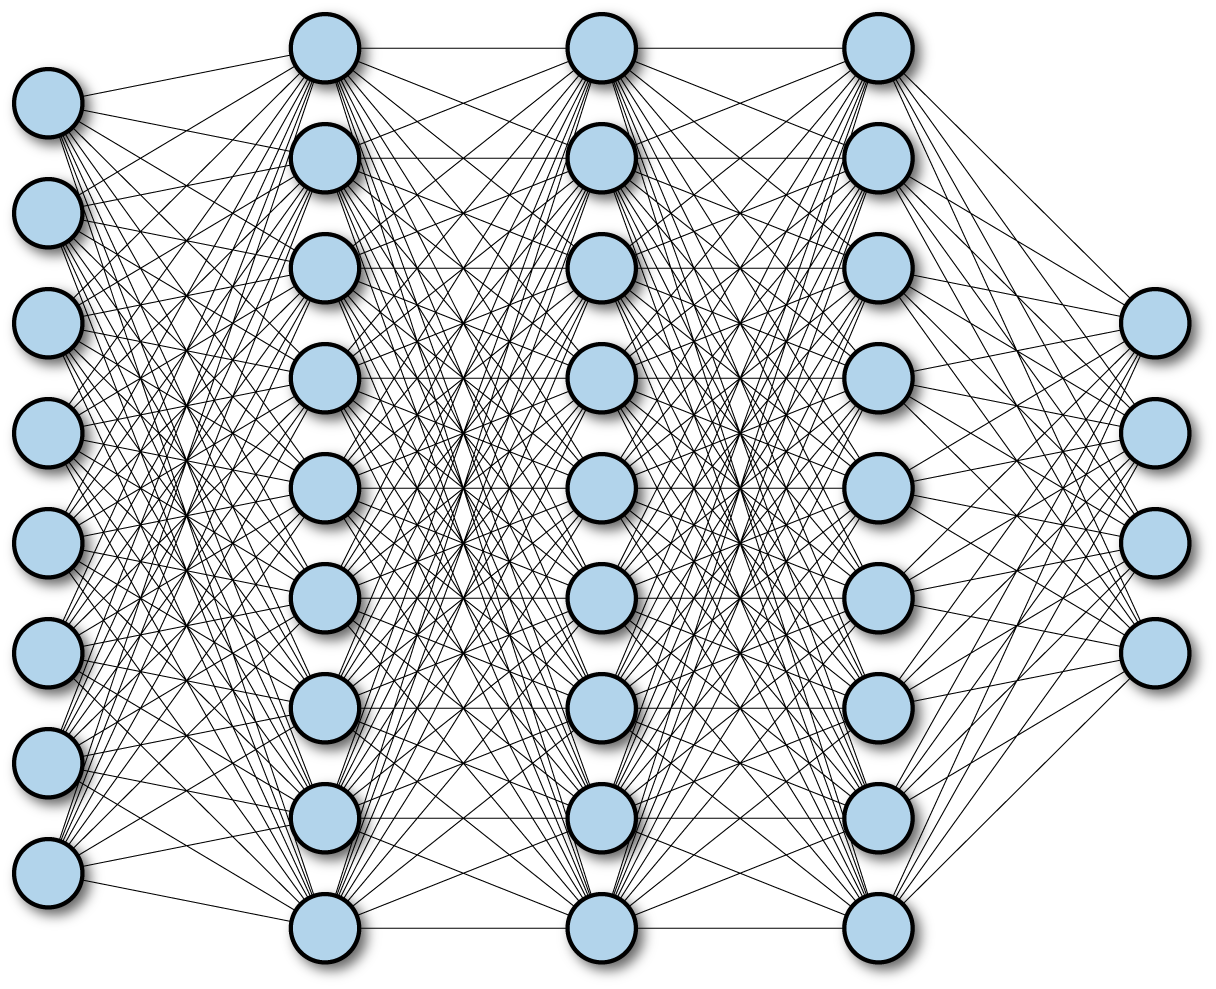
\includegraphics[width=0.8\textwidth]{fc}
  \caption{Full connected neural network}
  \label{fig:fc}
\end{figure}



%%% Local Variables:
%%% mode: latex
%%% TeX-master: "deep-learning"
%%% End:


\chapter{CNN}

CNN stands for convolutional neural network.
Convolutional networks are neural networks that have convolutional layers.
A typical convolutional layer consists of three stages:
\begin{enumerate}
\item convolution stage: affine transform
\item detector stage: nonlinearty
\item pooling stage
\end{enumerate}

\section{Convolution}

\begin{equation}
  \label{eq:convolution}
  s(t) = \int x(a)w(t-a)da.
\end{equation}

This operation is called \keyword{convolution}.
The convolution operation is typically denoted with an asterisk:
\begin{equation}
  s(t) = (x*w)(t).
\end{equation}

In convolutional network terminology, the first argument (in this example, the function $x$) to the convolution is often referred to as the \keyword{input}, and the second argument (int this example, the function $w$) as the \keyword{kernel}.
The output is sometimes referred to as the \keyword{feature map}.

If we assume that $x$ and $w$ are defined only on integer $t$, we can define the discrete convolution:
\begin{equation}
  \label{eq:discrete-convolution}
  s(t) = (x*w)(t) = \sum_{a=-\infty}^{\infty} x(a)w(t-a).
\end{equation}

We often use convolutions over more than one axis at a time.
For example, if we use a two-dimensinal image $I$ as our input, we probably also want to use a two-dimensional kernel $K$:
\begin{equation}
  S(i,j) = (I*K)(i,j) = \sum_m\sum_n I(m,n)K(i-m,j-n).
\end{equation}


The following formula can be used to calculate the output dimension.
\begin{gather}
  h_{o} = \frac{h_{i} - h_{k}}{h_{s}} + 1\\
  w_{o} = \frac{w_{i} - w_{k}}{w_{s}} + 1
\end{gather}
where \(h_{o}\) is the output height, \(h_{i}\) is the input height, \(h_{k}\) is the kernel height, \(h_{s}\) is the stride height, \(w_{o}\) is the output width, \(w_{i}\) is the input width, \(w_{k}\) is the kernel width, \(w_{s}\) is the stride width.

The convolution operation is shown in Figure \ref{fig:conv-op}.
\begin{figure}[!htbp]
  \centering
  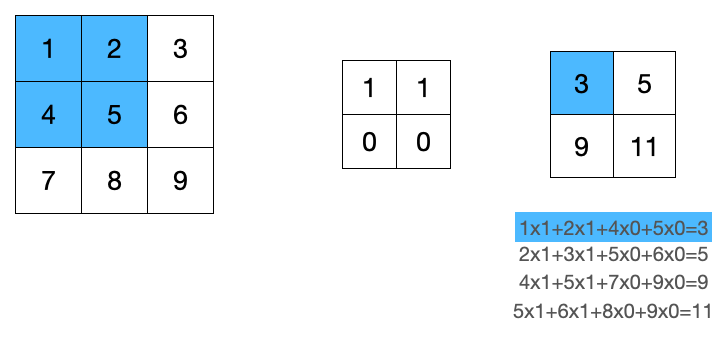
\includegraphics[width=0.8\textwidth]{conv}
  \caption{Convoluation operation}
  \label{fig:conv-op}
\end{figure}
\section{Properties}

CNN leverages three important ideas:
\begin{itemize}
\item sparse interaction.
\item parameter sharing.
\item equivariant representations.
\end{itemize}

\subsection{Sparse interaction}

This is accomplished by making the kernel smaller than the input.


\subsection{Parameter sharing}

In convolutional layers, the same parameter defined in one kernel are used at every position of the input.


\subsection{Equivariant representations}

In the case of convolution, the particular form of a parameter sharing causes the layer to have a property called \keyword{equivariance} to translation.
To say a function is equivariant means that if the input changes, the output changes in the same way.




\section{ Pooling}


A pooling function replaces the output of the net at a certain location with a summary statistic of the nearby outputs.
For example, the max pooling oeration reports the maximum output within a rectangular neighborhood.
Pooling helps to make the representation approximately invariant to small translations of the input.
Invariant to translation means that if we translate the input by a small amount, the values of most of the pooled outputs do not change.

The following formula can be used to calculate the output dimension.
\begin{gather}
  h_{o} = \frac{h_{i} - h_{k}}{h_{s}} + 1\\
  w_{o} = \frac{w_{i} - w_{k}}{w_{s}} + 1
\end{gather}
where \(h_{o}\) is the output height, \(h_{i}\) is the input height, \(h_{k}\) is the pooling height, \(h_{s}\) is the stride height, \(w_{o}\) is the output width, \(w_{i}\) is the input width, \(w_{k}\) is the pooling width, \(w_{s}\) is the stride width.


%%% Local Variables:
%%% mode: latex
%%% TeX-master: "machine-learning"
%%% End:


\chapter{Metric}
\label{cha:metric}

\begin{table}[H]
  \centering
  \begin{tabular}{ll|ll}
    \toprule
    \multicolumn{2}{l}{} & \multicolumn{2}{c}{Real value}\\
    \multicolumn{2}{l}{} & positive & negative \\
    \midrule
    \multirow{2}{*}{Predict value} & positive & true positive & false positive\\
    & negative & false negative & true negative\\
    \bottomrule
  \end{tabular}
  \caption{Confusion matrix}
  \label{tab:metric}
\end{table}

\section{Precision}
\label{sec:precision}



\begin{equation}
  \label{eq:2}
  \mbox{precision} = \frac{\mbox{TP}}{\mbox{TP} + \mbox{FP}}
\end{equation}


Of all the predicted positive values, the ratio of the true positive values (the real value is positive and the predicted value is positive).



\section{Recall}
\label{sec:recall}



\begin{equation}
  \label{eq:3}
  \mbox{recall} = \frac{\mbox{TP}}{\mbox{TP} + \mbox{FN}}
\end{equation}


Of all the real positive values, the ratio of the true positive values.


\section{Accuracy}
\label{sec:accuracy}

\begin{equation}
  \label{eq:4}
  \mbox{accuracy} = \frac{\mbox{TP} + \mbox{TN}}{\mbox{TP} + \mbox{TN} + \mbox{FP} + \mbox{FN}}
\end{equation}

Of all the values, the ratio of correctly predicted values.
The disadvantage is that it is not suitable for unbalanced data.


\section{F-score}
\label{sec:f-score}

\begin{equation}
  \label{eq:5}
  \text{F} = \frac{(\alpha^{2}+1) \times \text{precision} \times \text{recall}}{\alpha^{2} \times \text{precision} + \text{recall}}
\end{equation}


When determining the value of the parameter \(\alpha\), if we pay more attention to recall (compared to precision), we should choose a larger \(\alpha\).
The F-1 score is the expression when \(\alpha = 1\) 
%%% Local Variables:
%%% mode: latex
%%% TeX-master: "machine-learning"
%%% End:


\chapter{Regularization}
\label{cha:regularization}

We train model on training data but use test data (not used to train the model) to test out model.
The ability to perform on test data is called \keyword{generalization}.
We can use model on test data because we assume that the train data and the test has the same probability distribution (i.e. they have relationship).


\keyword{Regularization} is any modification we make to a learnining algorithm that is intended to reduce its generalization error.

In practice, it is very difficult to find a model with the right number of parameters.
Indeed, we often use a larger model that has been regularized appropriately.
\section{Parameter norm penalties}
\label{sec:param-norm-penalt}


Parameter norm penalties ($\Omega(\bm{\theta})$) can be added to the object function \(J\) to limit the capacity of the model.

\begin{equation}
  \label{eq:norm-penalties}
  \tilde{J}(\bm{\theta;X,y}) = J(\bm{\theta,X,y}) + \alpha \Omega(\bm{\theta})
\end{equation}


\subsection{$L^2$ Parameter Regularization}

The $L^2$ parameter norm penalty commonly known as \keyword{weight decay}.
\begin{equation}
  \label{eq:12}
  \Omega(\bm{\theta}) = \frac{1}{2} ||\bm{w}||_2^2
\end{equation}

Where \(\bm{w}\) is the model parameter matrix.

\subsection{$L^1$ Regularization}

$L^1$ regularization on the model parameter $\bm{w}$ is defined as
\begin{equation}
  \label{eq:l1}
  \Omega(\bm{\theta}) = ||\bm{w}||_1
\end{equation}

\section{Dataset Augmentation}

The best way to make a machine learning model generalize better is to train it on more data.
Of course, in practice, the amount of data we have is limited.
One way to get around this problem is to create fake data and add it to the training set.
Dataset augmentation has been a particular effective technique for a specific classification problem: object recognition.



\section{Early stopping}
\label{sec:early-stopping}


Early stopping is used to avoid overfit.

The algorithm terminates when no parameters have improved over the best recorded validation error for some pre-specified number of iterations.
This strategy is known as \keyword{early stopping}.
It is probably the most commonly used form of regularization in deep learning.


\section{Droupout}
\label{sec:droupout}



%%% Local Variables:
%%% mode: latex
%%% TeX-master: "machine-learning"
%%% End:


\chapter{Activation functions}
\label{cha:activation-functions}

Activation functions are usually added into neural network in order to help the network learn complex patterns.
Because many of the patterns we want to learn are non-linear, we usually add non-linear activation functions into neural network to add the ability to learn non-learn patterns.
Its function is to determine what information can be passed to the next neuron.


\section{Desirable features}
\label{sec:desirable-features}

\begin{itemize}
\item Differentiable. This is needed for optimization.
\item Low computational expense.
\item Zero-centered. 
\end{itemize}

\section{Sigmoid}
\label{sec:sigmoid}

\begin{equation}
  \label{eq:9}
  \text{sigmoid}(x)=\frac{1}{1+e^{-x}}
\end{equation}


It is no longer used in recent deep learning models because it is computationally expensive, causes vanishing gradient problem and not zero-centered.

\section{Tanh}
\label{sec:tanh}

\begin{equation}
  \label{eq:13}
  \tanh(x)=\frac{e^x-e^{-x}}{e^x+e^{-x}}=\frac{e^{2 x}-1}{e^{2 x}+1}
\end{equation}

Comparing to sigmoid, it solve the not zero-centered problem.

\section{ReLU}
\label{sec:relu}

\begin{equation}
  \label{eq:15}  
  \text{relu}(x)=\max (0, x)
\end{equation}

This is a widely used activation function.


\section{Leaky ReLU}
\label{sec:leaky-relu}

\begin{equation}
  \label{eq:16}
  \text{lrelu}(x)=\max (\alpha x, x)
\end{equation}


\section{Swish}
\label{sec:swish}

\begin{equation}
  \label{eq:17}
  \text{swish}(x)  = x * \operatorname{sigmoid}(x)  =x *(1+e^{-x})^{-1}
\end{equation}
%%% Local Variables:
%%% mode: latex
%%% TeX-master: "machine-learning"
%%% End:


\chapter{Machine learning process}
\label{cha:mach-learn-proc}

\begin{enumerate}
  
\item confirm your target
\item observe the data
\item preprocess the data it necessary
\item select the model
\item select the cost function
\item select the optimizer
\item train the model
\item fine-tune the model
\item predict the data using the model
\item deploy the model
\end{enumerate}
%%% Local Variables:
%%% mode: latex
%%% TeX-master: "machine-learning"
%%% End:



\part{Models}
\label{part:models}


\chapter{Diffusion}
\label{cha:diffusion}

Diffusion models are generative models, meaning that they are used to generate data similar to the data on which they are trained.
Fundamentally, diffusion models work by destroying training data through the successive addition of Gaussian noise, and then learning to recover the data by reversing this noising process.
After training, we can use the diffusion model to generate data by simply passing randomly sampled noise through the learned denoising process.




%%% Local Variables:
%%% mode: latex
%%% TeX-master: "machine-learning"
%%% End:



\part{Tools}
\label{part:tools}


\chapter{PyTorch}
\label{cha:pytorch}


%%% Local Variables:
%%% mode: latex
%%% TeX-master: "machine-learning"
%%% End:


\chapter{NumPy}
\label{cha:numpy}

\section{Load data}
\label{sec:load-data}

\begin{lstlisting}
import numpy as np

data = np.load('foo.npz')
\end{lstlisting}



%%% Local Variables:
%%% mode: latex
%%% TeX-master: "machine-learning"
%%% End:



\part{Practice}
\label{part:practice}


\chapter{Preprocessing}
\label{cha:preprocessing}

Preprocessing is not necessary.
We preprocess the data because we can not get what we want from the data directly.


\section{Not valued based data}
\label{sec:not-valued-based}

The computer can only process number-based data.
For not number-based data, we need to convert them into number-based data.
For example, convert a string into a number list.
For null values, we can drop them or compute them with other not null values.



\begin{lstlisting}
from sklearn.preprocessing import LabelBinarizer

data = ['dog', 'cat', 'dog', 'horse']
print('data: ', data)
binarizer = LabelBinarizer()
binarizer.fit(data)
print(binarizer.transform(data))
print(binarizer.transform(['dog']))

"""
data:  ['dog', 'cat', 'dog', 'horse']
[[0 1 0]
 [1 0 0]
 [0 1 0]
 [0 0 1]]
[[0 1 0]]
"""
\end{lstlisting}



%%% Local Variables:
%%% mode: latex
%%% TeX-master: "machine-learning"
%%% End:



\part{Projects}
\label{part:projects}

\part{Papers}
\label{part:papers}


\chapter{Deep Unsupervised Learning using Nonequilibrium Thermodynamics\protect{\cite{js2015deep}}}
\label{cha:deep-unsup-learn}


The algorithm consists of two trajectories: forward (inference) diffusion process and inverse (generative) diffusion process.
The forward diffusion process converts complex data distribution into a simple, tractable distribution and the inverse diffusion process learn a finite-time reversal of the forward diffusion process which define a generative model distribution.

\section{Algorithm}
\label{sec:algorithm}



\subsection{Forward trajectory}
\label{sec:forward-trajectory}
\begin{equation}
  \label{eq:18}
  \pi(\mathbf{y})=\int d \mathbf{y}^{\prime} T_\pi\left(\mathbf{y} \mid \mathbf{y}^{\prime} ; \beta\right) \pi\left(\mathbf{y}^{\prime}\right)
\end{equation}

Where \(\pi(\mathbf{y})\) is a well behaved (analyti- cally tractable) distribution.
\(T_\pi\left(\mathbf{y} \mid \mathbf{y}^{\prime} ; \beta\right)\) is a Markov diffusion kernel.
\(\beta\) is the diffusion rate.

\begin{equation}
  \label{eq:29}
  q\left(\mathbf{x}^{(t)} \mid \mathbf{x}^{(t-1)}\right)=T_\pi\left(\mathbf{x}^{(t)} \mid \mathbf{x}^{(t-1)} ; \beta_t\right)
\end{equation}

The forward trajectory, corresponding to starting at the data distribution and performing \(T\) steps of diffusion is
\begin{equation}
  \label{eq:30}
  q\left(\mathbf{x}^{(0 \cdots T)}\right)=q\left(\mathbf{x}^{(0)}\right) \prod_{t=1}^T q\left(\mathbf{x}^{(t)} \mid \mathbf{x}^{(t-1)}\right)
\end{equation}

Where \(q\left(\mathbf{x}^{(0)}\right)\) is the initial data distribution.

\subsection{Reverse Trajectory}
\label{sec:reverse-trajectory}
The generative distribution will be trained to describe the same trajectory, but in reverse,
\begin{equation}
  \label{eq:31}
  p\left(\mathbf{x}^{(T)}\right)=\pi\left(\mathbf{x}^{(T)}\right)
\end{equation}
\begin{equation}
  \label{eq:32}
  p\left(\mathbf{x}^{(0 \cdots T)}\right)=p\left(\mathbf{x}^{(T)}\right) \prod_{t=1}^T p\left(\mathbf{x}^{(t-1)} \mid \mathbf{x}^{(t)}\right)
\end{equation}

For both Gaussian and binomial diffusion, for continuous diffusion (limit of small step size $\beta$ ) the reversal of the diffusion process has the identical functional form as the forward process.
Since $q\left(\mathbf{x}^{(t)} \mid \mathbf{x}^{(t-1)}\right)$ is a Gaussian (binomial) distribution, and if $\beta_t$ is small, then $q\left(\mathbf{x}^{(t-1)} \mid \mathbf{x}^{(t)}\right)$ will also be a Gaussian (binomial) distribution.
The longer the trajectory the smaller the diffusion rate $\beta$ can be made.

During learning only the mean and covariance for a Gaussian diffusion kernel, or the bit flip probability for a binomial kernel, need be estimated.


\section{Model probability}
\label{sec:model-probability}

The probability the generative model assigns to the data is
\begin{equation}
  \label{eq:33}
p\left(\mathbf{x}^{(0)}\right)=\int d \mathbf{x}^{(1 \cdots T)} p\left(\mathbf{x}^{(0 \cdots T)}\right)  
\end{equation}

Naively this integral is intractable – but taking a cue from annealed importance sampling and the Jarzynski equality, we instead evaluate the relative probability of the forward and reverse trajectories, averaged over forward trajectories
\begin{equation}
  \label{eq:34}
\begin{aligned}
& p\left(\mathbf{x}^{(0)}\right)=\int d \mathbf{x}^{(1 \cdots T)} p\left(\mathbf{x}^{(0 \cdots T)}\right) \frac{q\left(\mathbf{x}^{(1 \cdots T)} \mid \mathbf{x}^{(0)}\right)}{q\left(\mathbf{x}^{(1 \cdots T)} \mid \mathbf{x}^{(0)}\right)} \\
&=\int d \mathbf{x}^{(1 \cdots T)} q\left(\mathbf{x}^{(1 \cdots T)} \mid \mathbf{x}^{(0)}\right) \frac{p\left(\mathbf{x}^{(0 \cdots T)}\right)}{q\left(\mathbf{x}^{(1 \cdots T)} \mid \mathbf{x}^{(0)}\right)} \\
&=\int d \mathbf{x}^{(1 \cdots T)} q\left(\mathbf{x}^{(1 \cdots T)} \mid \mathbf{x}^{(0)}\right) \cdot p\left(\mathbf{x}^{(T)}\right) \prod_{t=1}^T \frac{p\left(\mathbf{x}^{(t-1)} \mid \mathbf{x}^{(t)}\right)}{q\left(\mathbf{x}^{(t)} \mid \mathbf{x}^{(t-1)}\right)}
\end{aligned}  
\end{equation}


\section{Training}
\label{sec:training}

Training amounts to maximizing the model log likelihood,
\begin{equation}
  \label{eq:35}
\begin{aligned}
L= & \int d \mathbf{x}^{(0)} q\left(\mathbf{x}^{(0)}\right) \log p\left(\mathbf{x}^{(0)}\right) \\
= & \int d \mathbf{x}^{(0)} q\left(\mathbf{x}^{(0)}\right) \cdot 
 \log \left[\begin{array}{c}
\int d \mathbf{x}^{(1 \cdots T)} q\left(\mathbf{x}^{(1 \cdots T)} \mid \mathbf{x}^{(0)}\right) . \\
p\left(\mathbf{x}^{(T)}\right) \prod_{t=1}^T \frac{p\left(\mathbf{x}^{(t-1)} \mid \mathbf{x}^{(t)}\right)}{q\left(\mathbf{x}^{(t)} \mid \mathbf{x}^{(t-1)}\right)}
\end{array}\right],
\end{aligned}
\end{equation}


which has a lower bound provided by Jensen's inequality,
\begin{equation}
  \label{eq:37}
L \geq  \int d \mathbf{x}^{(0 \cdots T)} q\left(\mathbf{x}^{(0 \cdots T)}\right) \cdot  \log \left[p\left(\mathbf{x}^{(T)}\right) \prod_{t=1}^T \frac{p\left(\mathbf{x}^{(t-1)} \mid \mathbf{x}^{(t)}\right)}{q\left(\mathbf{x}^{(t)} \mid \mathbf{x}^{(t-1)}\right)}\right] .  
\end{equation}




for our diffusion trajectories this reduces to,
\begin{equation}
  \label{eq:36}
L  \geq K 
\end{equation}
\begin{equation}
  \label{eq:39}
  \begin{aligned}
K= & -\sum_{t=2}^T \int d \mathbf{x}^{(0)} d \mathbf{x}^{(t)} q\left(\mathbf{x}^{(0)}, \mathbf{x}^{(t)}\right) \\
& D_{K L}\left(q\left(\mathbf{x}^{(t-1)} \mid \mathbf{x}^{(t)}, \mathbf{x}^{(0)}\right)|| p\left(\mathbf{x}^{(t-1)} \mid \mathbf{x}^{(t)}\right)\right) \\
+ & H_q\left(\mathbf{X}^{(T)} \mid \mathbf{X}^{(0)}\right)-H_q\left(\mathbf{X}^{(1)} \mid \mathbf{X}^{(0)}\right)-H_p\left(\mathbf{X}^{(T)}\right)
  \end{aligned}
\end{equation}

where the entropies and KL divergences can be analytically computed. The derivation of this bound parallels the derivation of the log likelihood bound in variational Bayesian methods.

If the forward and reverse trajectories are identical, corresponding to a quasi-static process, then the inequality in Equation \ref{eq:36} becomes an equality.

Training consists of finding the reverse Markov transitions which maximize this lower bound on the log likelihood,
\begin{equation}
  \label{eq:38}
\hat{p}\left(\mathbf{x}^{(t-1)} \mid \mathbf{x}^{(t)}\right)=\underset{p\left(\mathbf{x}^{(t-1)} \mid \mathbf{x}^{(t)}\right)}{\operatorname{argmax}} K .  
\end{equation}


%%% Local Variables:
%%% mode: latex
%%% TeX-master: "machine-learning"
%%% End:



% Pages are numbered with Arabic numbers.
% Chapters generate a table of contents entry but don't get a number.
\backmatter{}
\cleardoublepage{}
\phantomsection{}
%\nocite{*}   % cite all in bibliography
\bibliographystyle{plain}       % % plain, unsrt, alpha, abbrv
\bibliography{refs}

\cleardoublepage{}
% just setting an anchor like \hypertarget{}{}
% fix the problem that anchor point to the previous section
\phantomsection{}                 
\printindex{}
\end{document}

%%% Local Variables:
%%% mode: latex
%%% TeX-master: t
%%% End:


